\documentclass[tikz,border=2pt]{standalone}
\usepackage{amsmath}
\usetikzlibrary{arrows.meta}
\begin{document}
% Batch-service queue (Exercise 4.6.9), lambda = 1, mu = 2: arrivals n -> n+1 for n < 3, batch
% completions 2 -> 0 and 3 -> 1; p = (4,6,2,1)/13. Box around state 1: in lambda p(0) + mu p(3) = 6/13 = out lambda p(1).
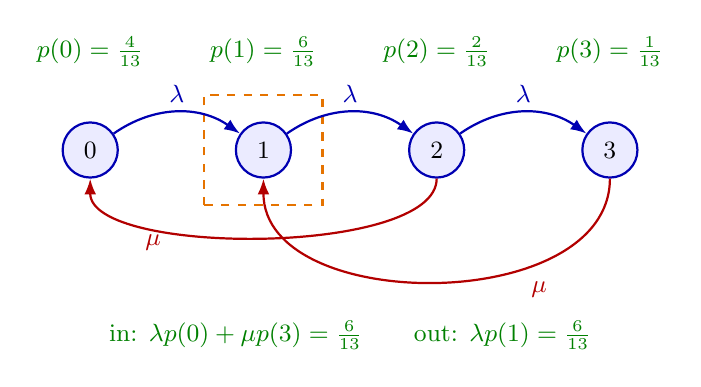
\begin{tikzpicture}[font=\small, >={Latex[length=2mm]},
  st/.style={circle, draw=blue!70!black, thick, fill=blue!8, minimum size=7mm, inner sep=0pt}]
  \foreach \n in {0,...,3} \node[st] (s\n) at (2.2*\n,0) {$\n$};
  % box around state 1
  \draw[orange!90!black, thick, dashed] (2.2-0.75,-0.7) rectangle (2.2+0.75,0.7);
  % arrivals
  \foreach \n/\m in {0/1,1/2,2/3}
    \draw[->, thick, blue!70!black] (s\n) to[bend left=35] node[above] {$\lambda$} (s\m);
  % batch completions
  \draw[->, thick, red!70!black] (s2.south) .. controls (4.4,-1.35) and (0,-1.35) .. (s0.south);
  \draw[->, thick, red!70!black] (s3.south) .. controls (6.6,-2.1) and (2.2,-2.1) .. (s1.south);
  \node[red!70!black, anchor=north] at (0.8,-0.95) {$\mu$};
  \node[red!70!black, anchor=north] at (5.7,-1.55) {$\mu$};
  % stationary probabilities
  \foreach \n/\p in {0/\tfrac{4}{13},1/\tfrac{6}{13},2/\tfrac{2}{13},3/\tfrac{1}{13}}
    \node[green!50!black] at (2.2*\n,1.25) {$p(\n)=\p$};
  % flow summary
  \node[green!50!black] at (3.3,-2.35) {in: $\lambda p(0)+\mu p(3)=\tfrac{6}{13}$\qquad out: $\lambda p(1)=\tfrac{6}{13}$};
\end{tikzpicture}
\end{document}
